\documentclass{article}
\usepackage{graphicx}

%\newcommand{\test}{\input{id.txt}\unskip}
%\graphicspath{{/var/www/html/nrb/Mapps/Conabio/reportesPDF/LaTeX/341810900dir/}}
\graphicspath{{./LaTeX/341810900dir/}}
%\graphicspath{{/var/www/html/nrb/Mapps/Conabio/reportesPDF/LaTeX/341810900dir/}}


\begin{document}

	\title{Introduction to \LaTeX{}}
	\author{Author's Name}

	\maketitle

	\begin{abstract}
		The abstract text goes here.
	\end{abstract}

	\section{Introduction}
		Here is the text of your introduction.

	\begin{equation}
	    \label{simple_equation}
	    \alpha = \sqrt{ \beta }
	\end{equation}

	\subsection{Subsection Heading Here}
		Write your subsection text here.
		LaTeX/\input{id.txt}

	\begin{figure}
	\centering
	
\includegraphics[width=3.0in]{1}
	\end{figure}

	% \begin{figure}
	%     \centering
	%     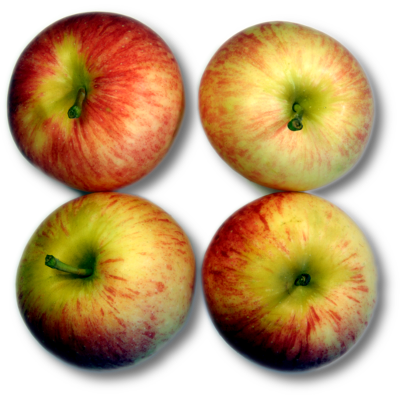
\includegraphics[width=3.0in]{LaTeX/images/img}
	%     %
\includegraphics[width=3.0in]{/var/www/html/nrb/Mapps/Conabio/reportesPDF/1.png}
	%     %\includegraphics[width=3.0in]{/var/www/html/nrb/Mapps/Conabio/reportesPDF/LaTeX/\input{id.txt}\unskip/1}
	%     %\input{../LULCC/TempTables/Country.txt}
	%     \caption{Test Image}
	%    	\label{Test Image}

	% \end{figure}

	\section{Conclusion}
	Write your conclusion here.

\end{document}